\documentclass[11pt]{report}
\usepackage{graphicx}
\usepackage{pgfplots}
\usepackage{amsfonts}
\usepackage[all]{xy}
\usepackage{amsmath}
\usepackage{amssymb}
\usepackage{tikz}
\usepackage{forest}
\usepackage{tikz}
\usepackage{caption}
\usepackage{listings}
\usepackage{hyperref}
\usepackage{float}
% we want ER + above/below + left/right
\usetikzlibrary{er,positioning}
\usepackage{hyperref}
%Gummi|065|=)
\title{\textbf{MonitoringBox Manual}\\Raspberry pi}
\author{Team MonitoringBox}
\date{2017}
\begin{document}


\definecolor{mygreen}{rgb}{0,0.6,0}
\definecolor{mygray}{rgb}{0.5,0.5,0.5}
\definecolor{mymauve}{rgb}{0.58,0,0.82}
\definecolor{bg}{rgb}{0.9,0.9,0.9}

% https://en.wikibooks.org/wiki/LaTeX/Source_Code_Listings
\lstset{ %
  backgroundcolor=\color{bg},   % choose the background color
  basicstyle=\footnotesize,        % size of fonts used for the code
  breaklines=true,                 % automatic line breaking only at whitespace
  captionpos=b,                    % sets the caption-position to bottom
  commentstyle=\color{mygreen},    % comment style
  escapeinside={\%*}{*)},          % if you want to add LaTeX within your code
  keywordstyle=\color{blue},       % keyword style
  stringstyle=\color{mymauve},     % string literal style
  framesep=10pt,xleftmargin=10pt,xrightmargin=10pt
}

\maketitle

\tableofcontents{}

\chapter{Introduction}
	The base of the monitoring box is the Raspberry Pi, as you can see figure 1.1\\\\
	\begin{figure}[h!]
		\centering
		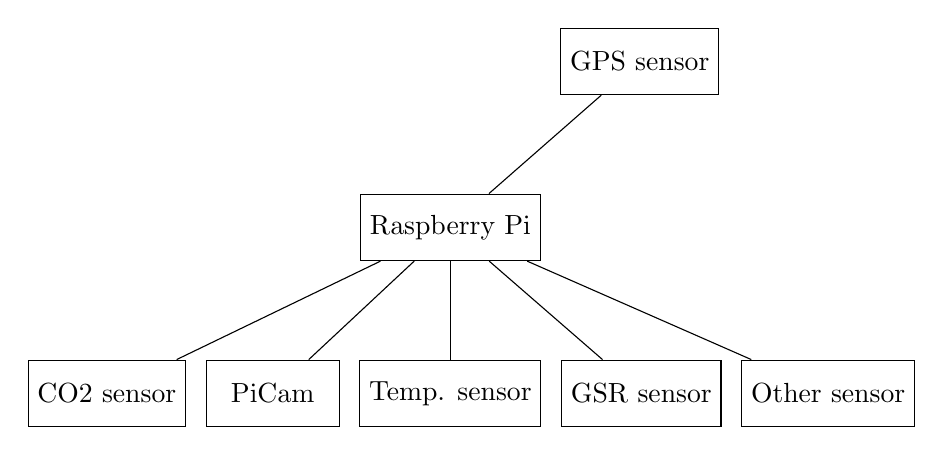
\begin{tikzpicture}[auto,node distance=1.25cm and 0.25cm]
			\node[entity] (nodeRoot) {Raspberry Pi};
			\node[entity] (nodeGPS) [above right = of nodeRoot]	{GPS sensor};
			\node[entity] (nodeC) [below = of nodeRoot]	{Temp. sensor};
			\node[entity] (nodeL) [left = of nodeC]	{PiCam};
			\node[entity] (nodeLL) [left = of nodeL]	{CO2 sensor};
			\node[entity] (nodeR) [right = of nodeC]	{GSR sensor};
			\node[entity] (nodeRR) [right = of nodeR]	{Other sensor};
			\path (nodeRoot) edge node {} (nodeC);
			\path (nodeRoot) edge node {} (nodeL);
			\path (nodeRoot) edge node {} (nodeLL);
			\path (nodeRoot) edge node {} (nodeR);
			\path (nodeRoot) edge node {} (nodeRR);
			\path (nodeRoot) edge node {} (nodeGPS);
		\end{tikzpicture}
		\caption{Example of setup of sensors connected to the Pi.}
	\end{figure}
	
	The Raspberry Pi contains the software that knows how to interpret the sensor data, allows for exporting of the data and converting it to the wanted format. The user can connect to the Raspberry Pi via WiFi.
\chapter{Requirements/parts}
	The hardware and software described in this chapter are required to complete the MonitoringBox.
	\section{Hardware}
		The hardware required for the base of the MonitoringBox:
		\begin{list}{-}
			\item Raspberry Pi 3 (https://www.raspberrypi.org/products/raspberry-pi-3-model-b/)
			\item 
			\item Touchscreen (...) @todo
			\item Casing (optional) (see github .... ) @todo
		\end{list}
	\section{Software}
		The operating system used for the Raspberry Pi is Raspbian (lite) which can be download from https://www.raspberrypi.org/downloads/raspbian/
		
		The management software that is required for the MonitoringBox to function is available on https://github.com/pjotrscholtze/MonitoringBox

\chapter{Installation}
	The installation of the base of the MonitoringBox can be divided into two parts: the hardware part and software part. 
	\section{Hardware}
		@todo show how to insert the SD card and put it into the box, and how to connect the display (don forget the jumper on the screen)
	\newpage
	\section{OS}
		\subsection{Download}
			Download Raspbian Lite from: 
			\href{https://www.raspberrypi.org/downloads/raspbian/}{https://www.raspberrypi.org/downloads/raspbian/}
			\begin{figure}[ht]
				\centering
				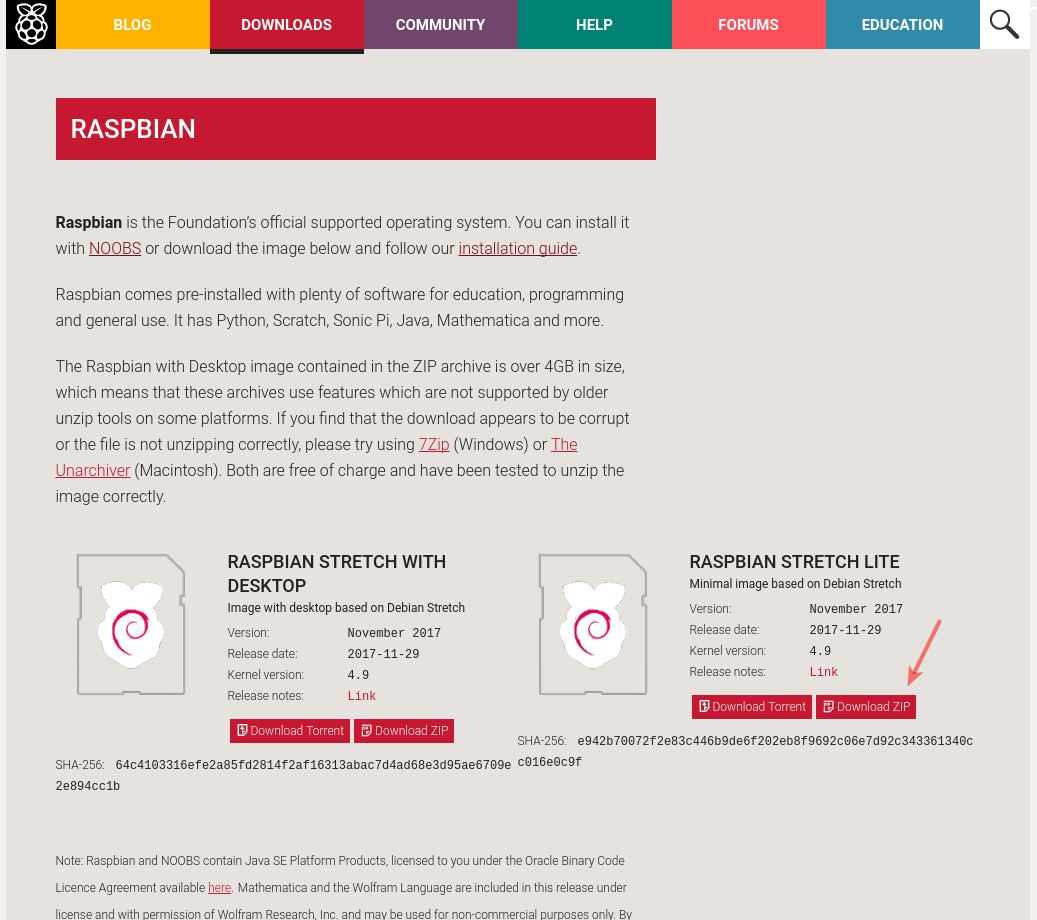
\includegraphics[width=0.75\textwidth]{images/pi/download_raspbian.png} 
				\caption{Download Raspbian Lite}
			\end{figure}
			\newpage
		And download Etcher from: \href{https://etcher.io/}{https://etcher.io/} (works on Windows, Linux and OS X).

			\begin{figure}[ht]
				\centering
				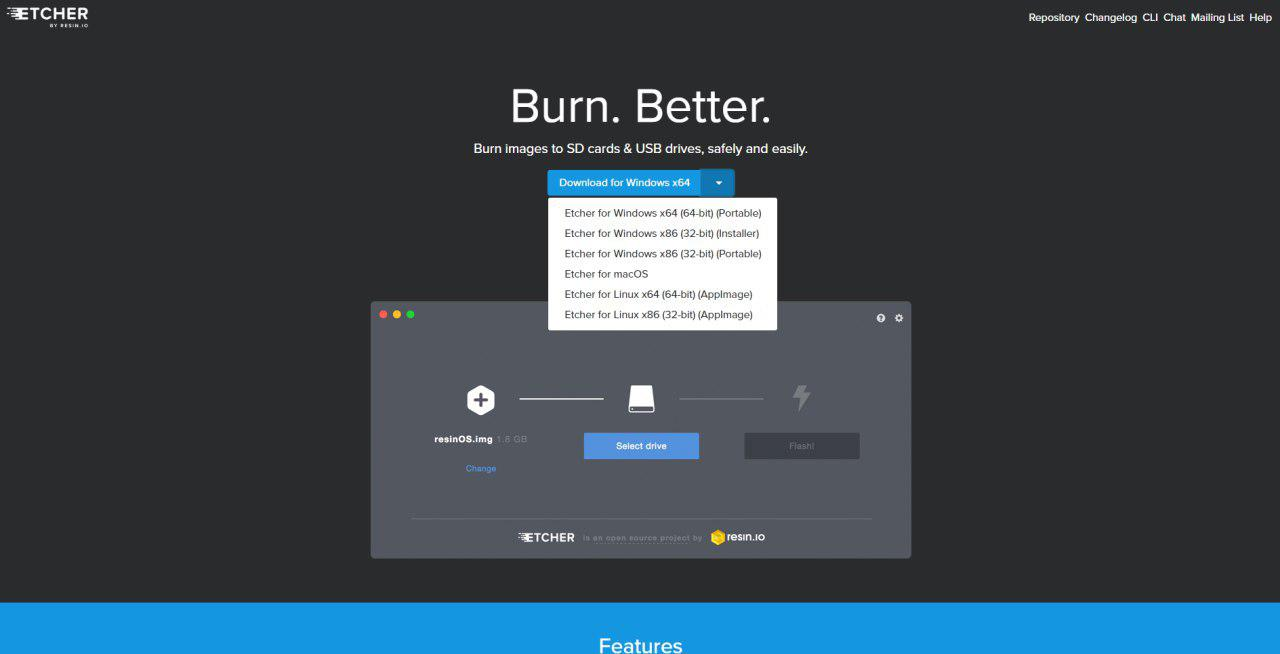
\includegraphics[width=0.75\textwidth]{images/pi/install_etcher_1.jpg} 
				\caption{Download Etcher}
			\end{figure}
		\subsection{Flash the SD card}
			Start Etcher. And press "Select image"
			\begin{figure}[ht]
				\centering
				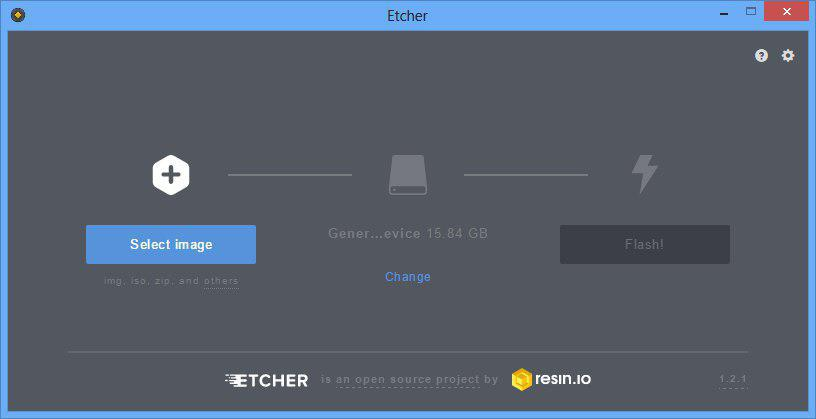
\includegraphics[width=0.75\textwidth]{images/pi/install_etcher_2.jpg} 
				\caption{Etcher start up state.}
			\end{figure}
			\newpage
			Go to the location of the downloaded Raspbian file.
			\begin{figure}[H]
				\centering
				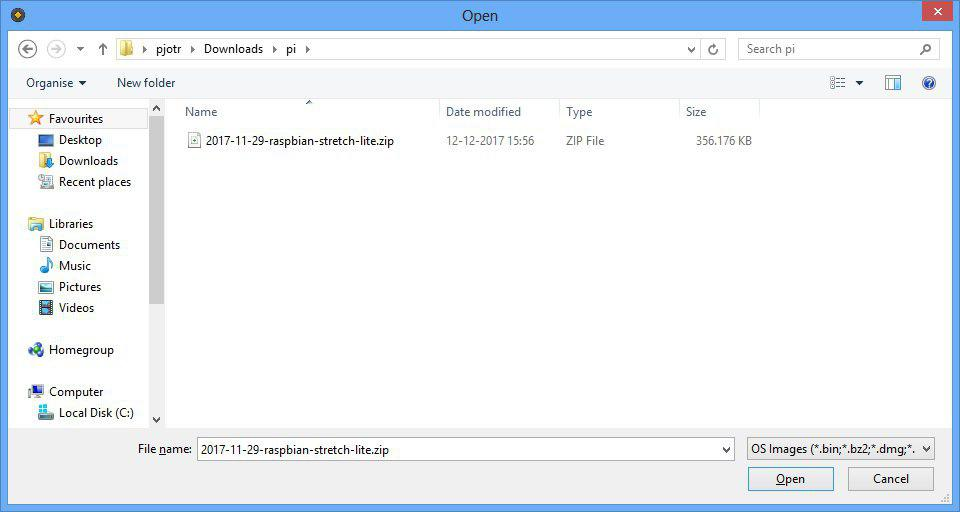
\includegraphics[width=0.75\textwidth]{images/pi/install_etcher_3.jpg} 
				\caption{The Mikroe Gas Detector}
			\end{figure}
			Select the SD card.
			\begin{figure}[ht]
				\centering
				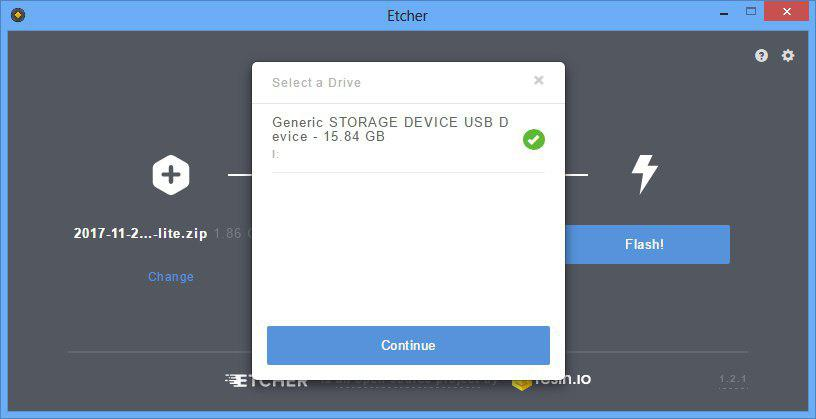
\includegraphics[width=0.75\textwidth]{images/pi/install_etcher_4.jpg} 
				\caption{The Mikroe Gas Detector}
			\end{figure}
			\newpage
			And press "Flash!"
			\begin{figure}[ht]
				\centering
				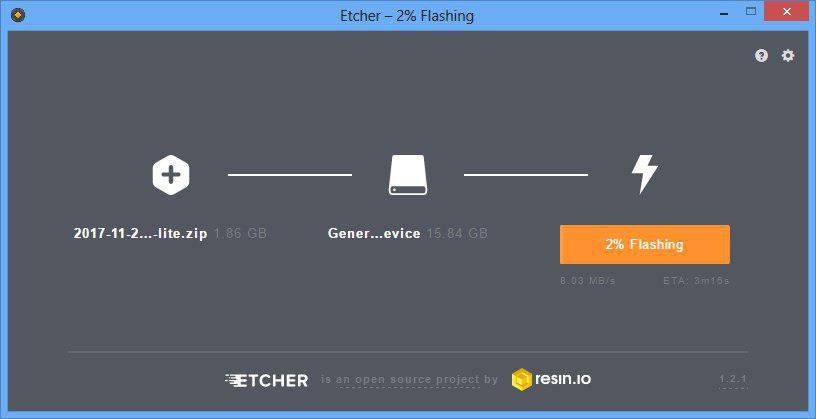
\includegraphics[width=0.75\textwidth]{images/pi/install_etcher_5.jpg} 
				\caption{The Mikroe Gas Detector}
			\end{figure}
			This will take sometime. Afterwards the following screen will appear:
			\begin{figure}[ht]
				\centering
				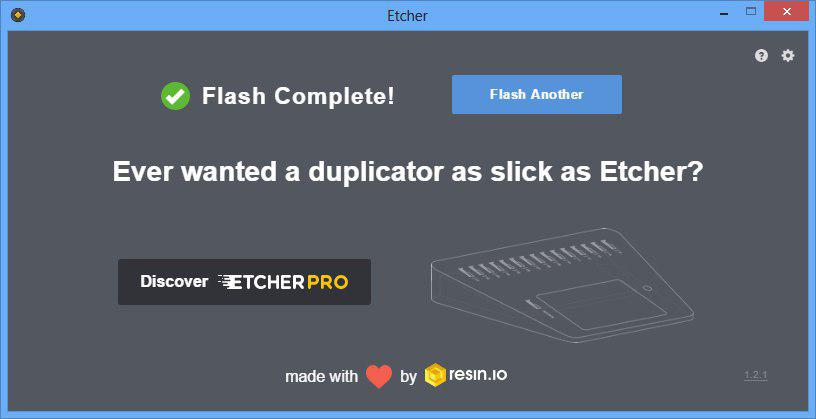
\includegraphics[width=0.75\textwidth]{images/pi/install_etcher_6.jpg} 
				\caption{The Mikroe Gas Detector}
			\end{figure}
			This screen means you can remove the SD card.
			\newpage
			And plug it into the Pi.
			\begin{figure}[ht]
				\centering
				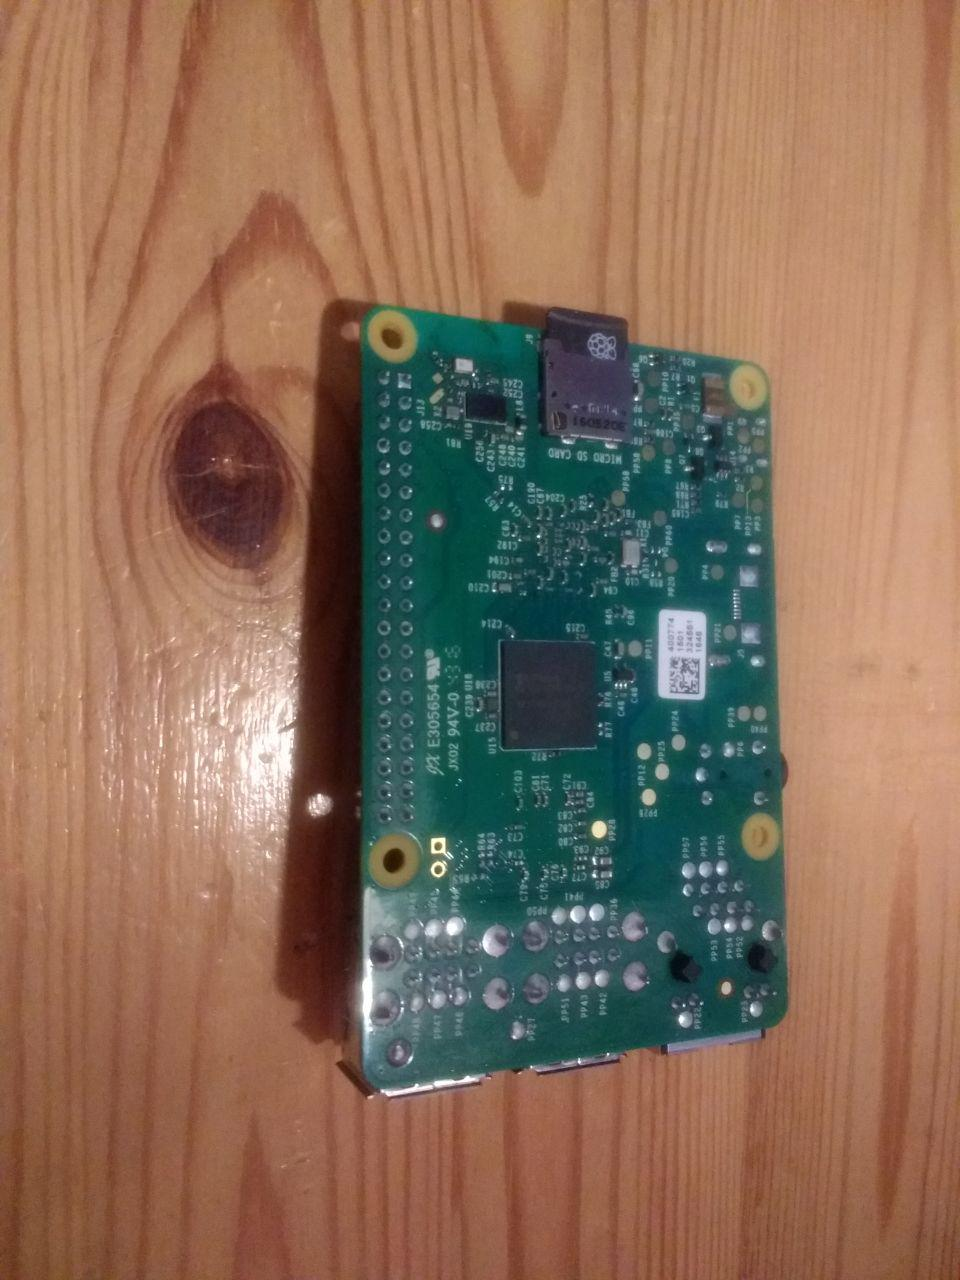
\includegraphics[width=0.45\textwidth]{images/pi/install_sd_1.jpg}
				\caption{The Mikroe Gas Detector}
			\end{figure}
			Attach all required cables (keyboard, HDMI for screen power and Ethernet).
			\begin{figure}[ht]
				\centering
				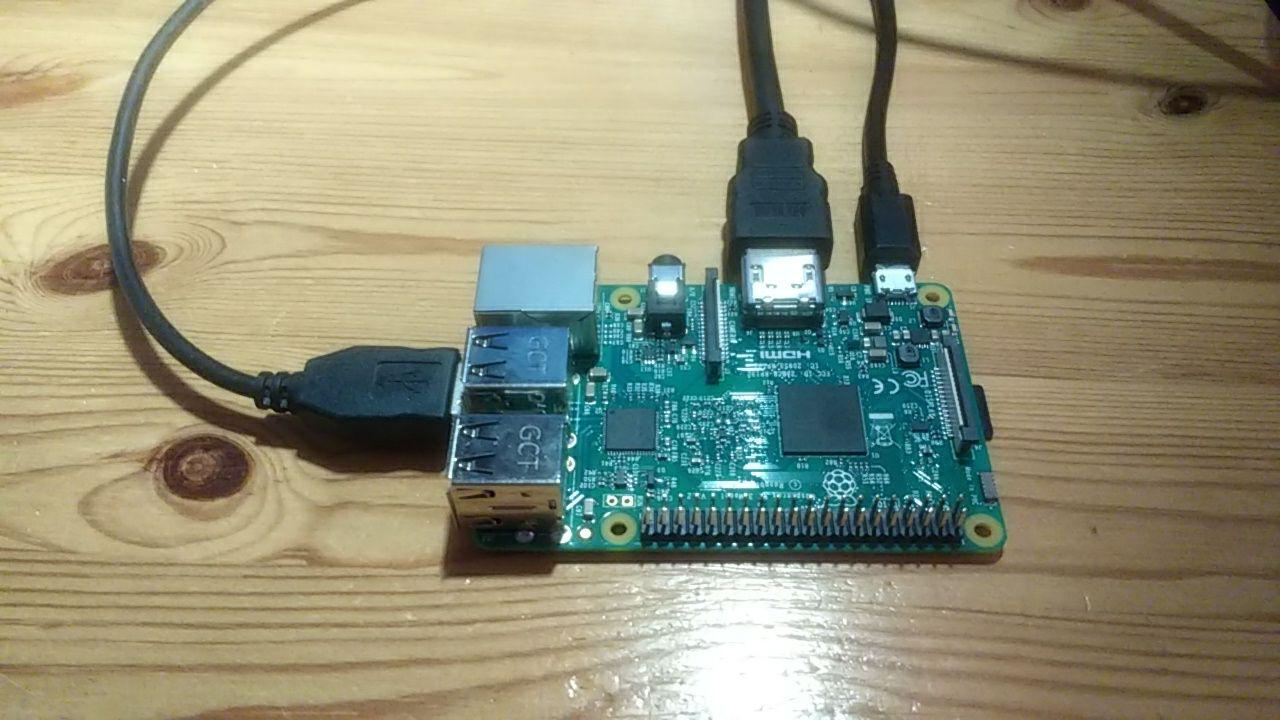
\includegraphics[width=0.6\textwidth]{images/pi/install_cables.jpg} 
				\caption{The Mikroe Gas Detector}
			\end{figure}
			\newpage
		\subsection{First boot}
			On first boot the system is going to show this screen and restart automatically.
			\begin{figure}[ht]
				\centering
				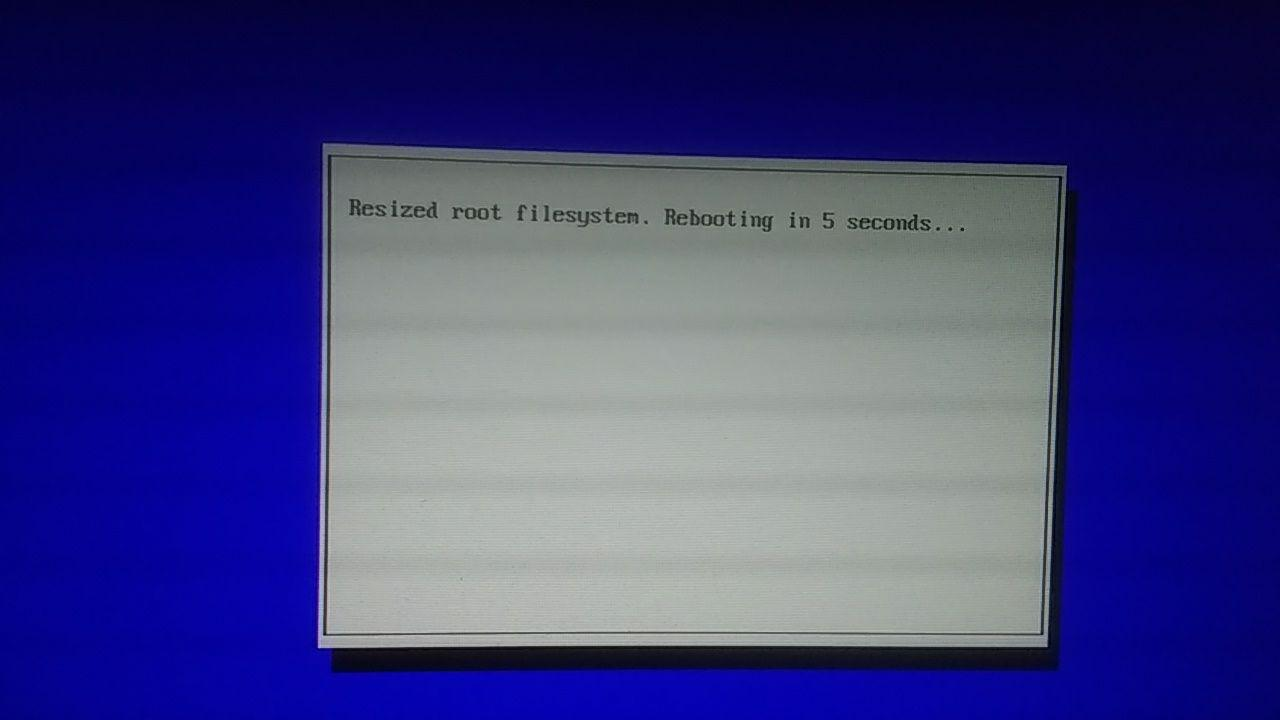
\includegraphics[width=0.75\textwidth]{images/pi/install_first_boot.jpg} 
				\caption{The Mikroe Gas Detector}
			\end{figure}\\
			When the following is visible you need to login in to the Pi. Default username is: pi and the default password is: raspberry
			\begin{figure}[ht]
				\centering
				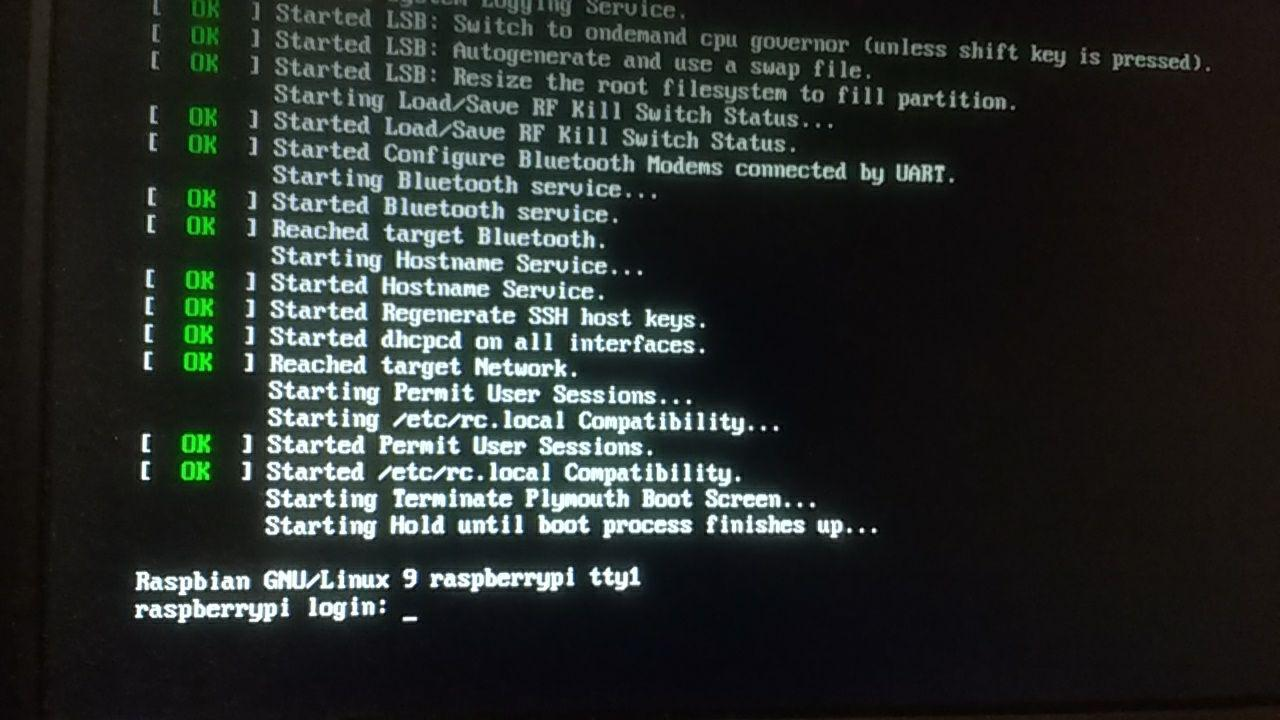
\includegraphics[width=0.75\textwidth]{images/pi/first_login.jpg} 
				\caption{The Mikroe Gas Detector}
			\end{figure}
			\newpage
			After logging in the following should show:
			\begin{figure}[ht]
				\centering
				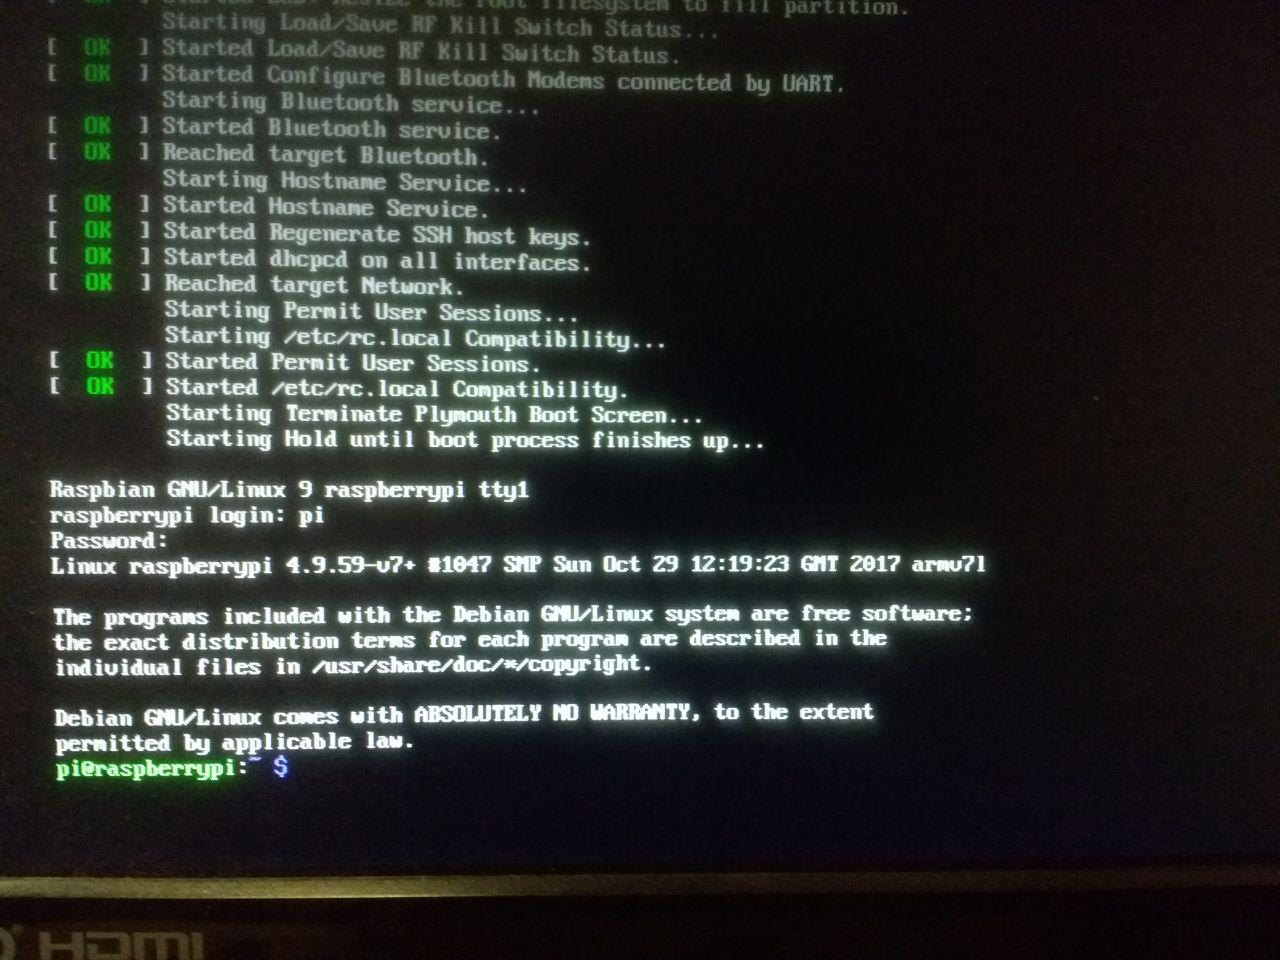
\includegraphics[width=0.6\textwidth]{images/pi/first_login_after_login.jpg} 
				\caption{The Mikroe Gas Detector}
			\end{figure}\\
			In here write the following command: sudo raspi-config
			\begin{figure}[ht]
				\centering
				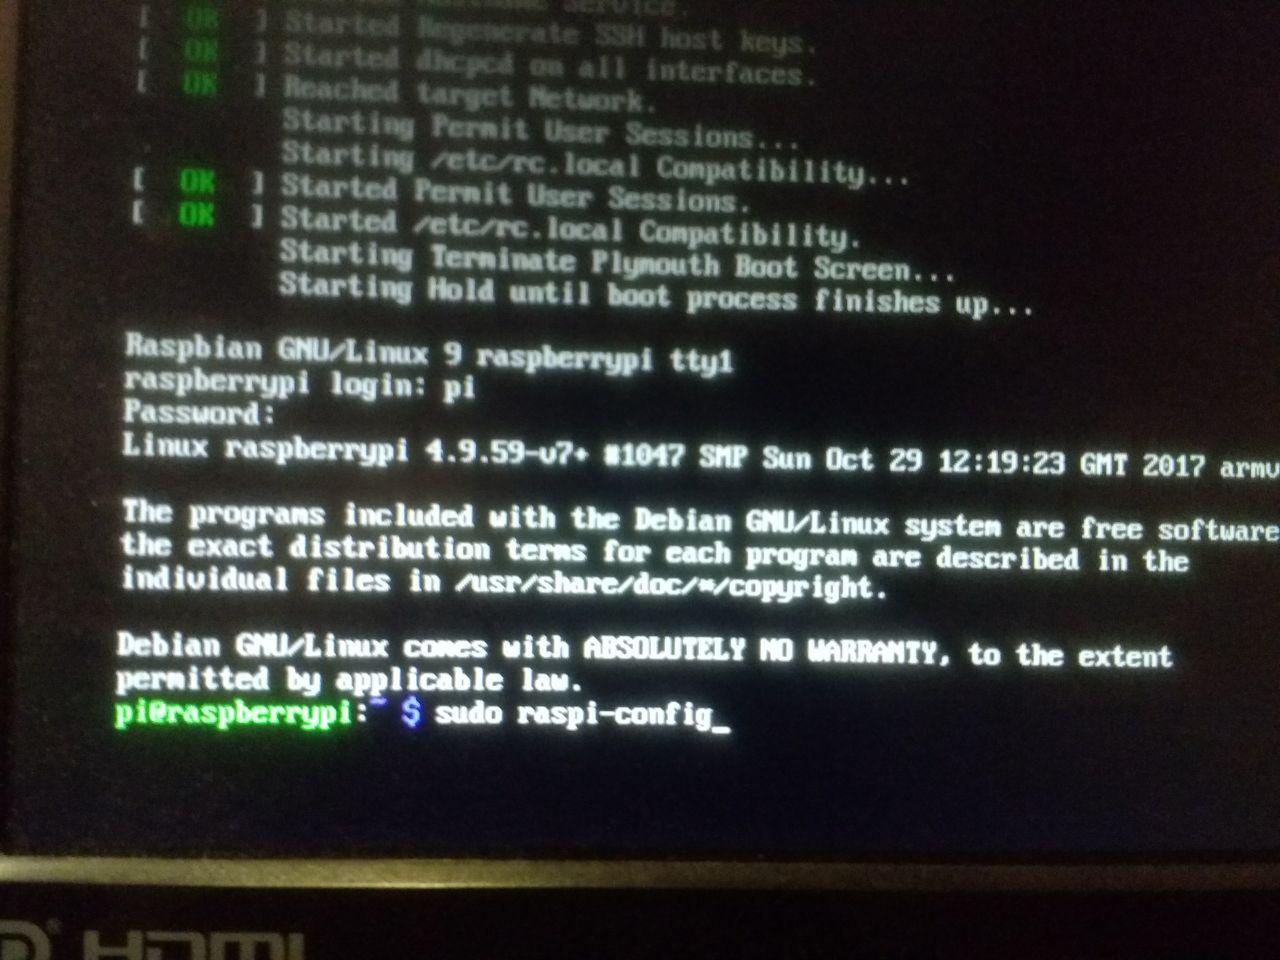
\includegraphics[width=0.6\textwidth]{images/pi/ssh_command.jpg} 
				\caption{The Mikroe Gas Detector}
			\end{figure}
			\newpage
			In the screen that just showed, go to the 5th option with the arrow keys, then enter:
			\begin{figure}[ht]
				\centering
				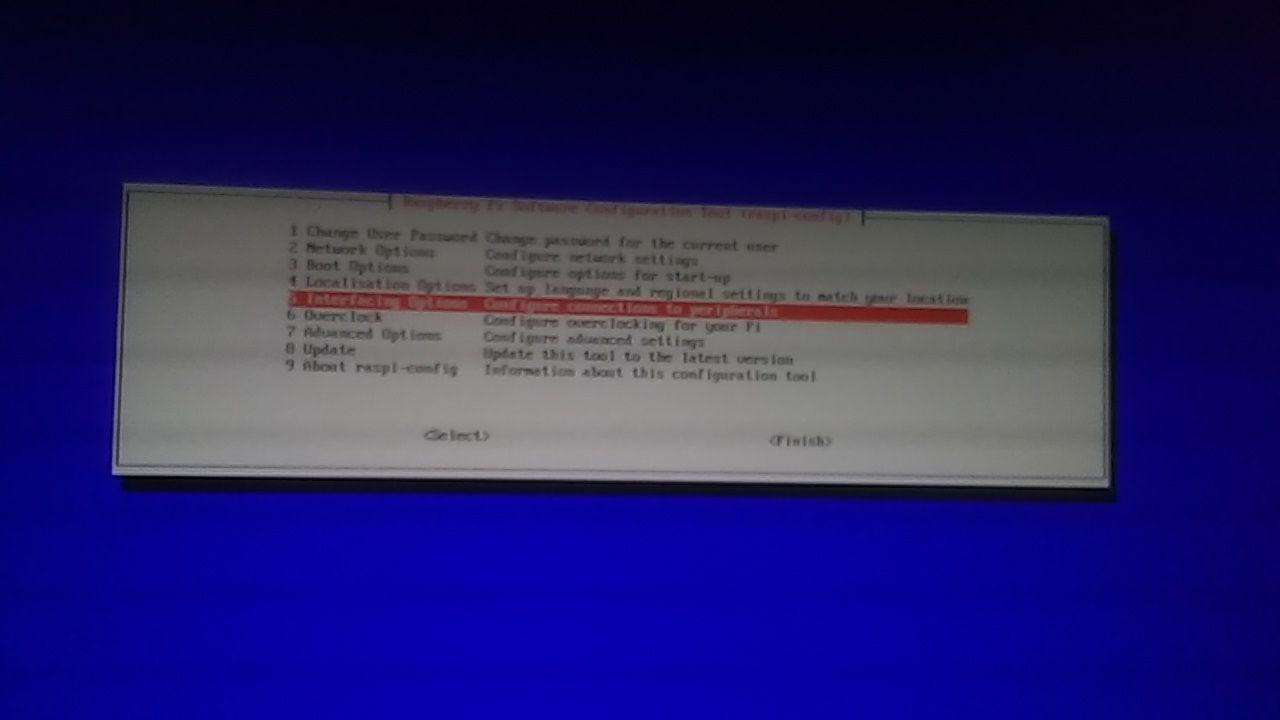
\includegraphics[width=0.75\textwidth]{images/pi/ssh_1.jpg} 
				\caption{The Mikroe Gas Detector}
			\end{figure}\\
			Select the the second option \textbf{SSH}:
			\begin{figure}[ht]
				\centering
				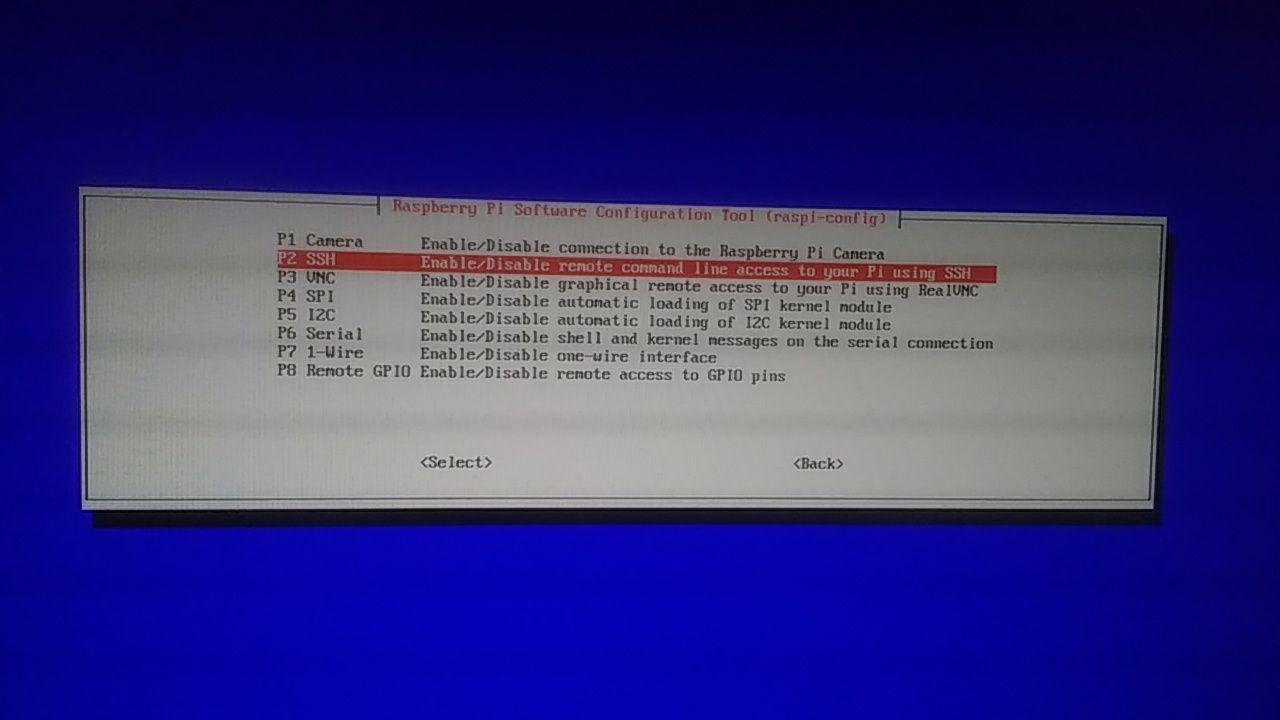
\includegraphics[width=0.75\textwidth]{images/pi/ssh_2.jpg} 
				\caption{The Mikroe Gas Detector}
			\end{figure}
			\newpage
			Enable the SSH server (select \textbf{Yes} and then press enter)
			\begin{figure}[ht]
				\centering
				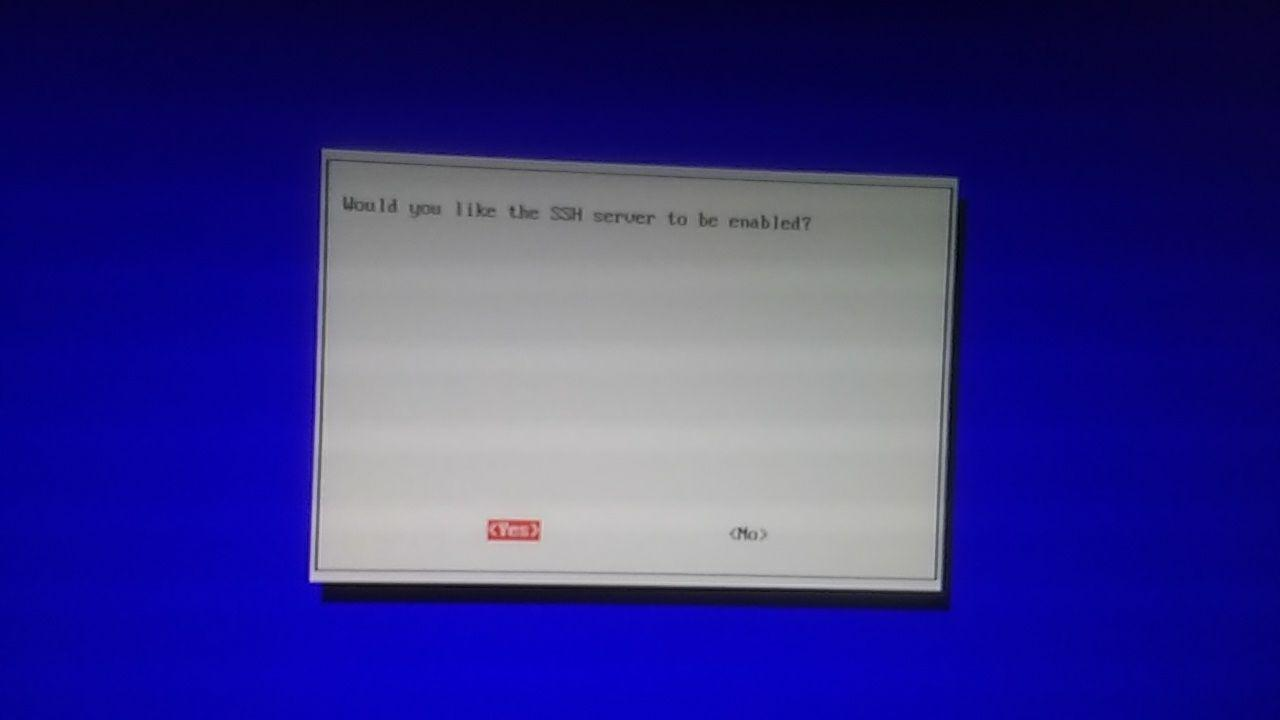
\includegraphics[width=0.75\textwidth]{images/pi/ssh_3.jpg} 
				\caption{The Mikroe Gas Detector}
			\end{figure}\\
			Press \textbf{Ok}
			\begin{figure}[ht]
				\centering
				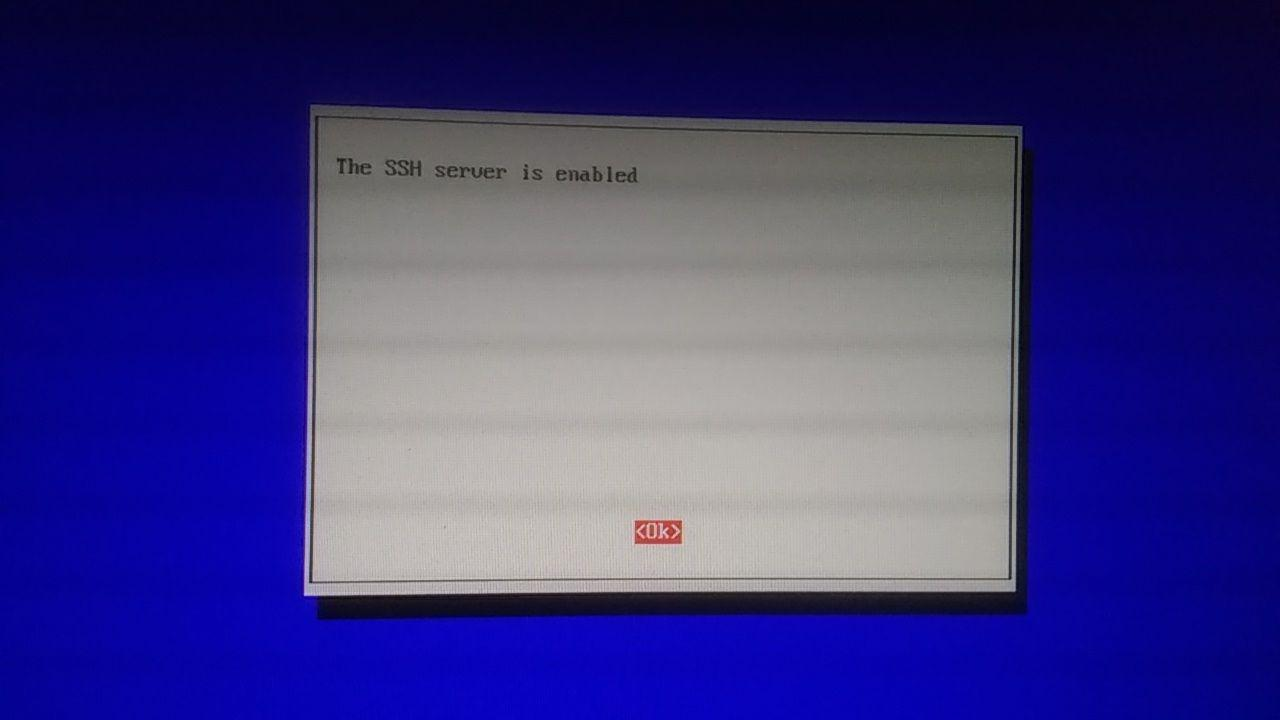
\includegraphics[width=0.75\textwidth]{images/pi/ssh_4.jpg} 
				\caption{The Mikroe Gas Detector}
			\end{figure}
			\newpage
			Finish the dialog (close it).
			\begin{figure}[ht]
				\centering
				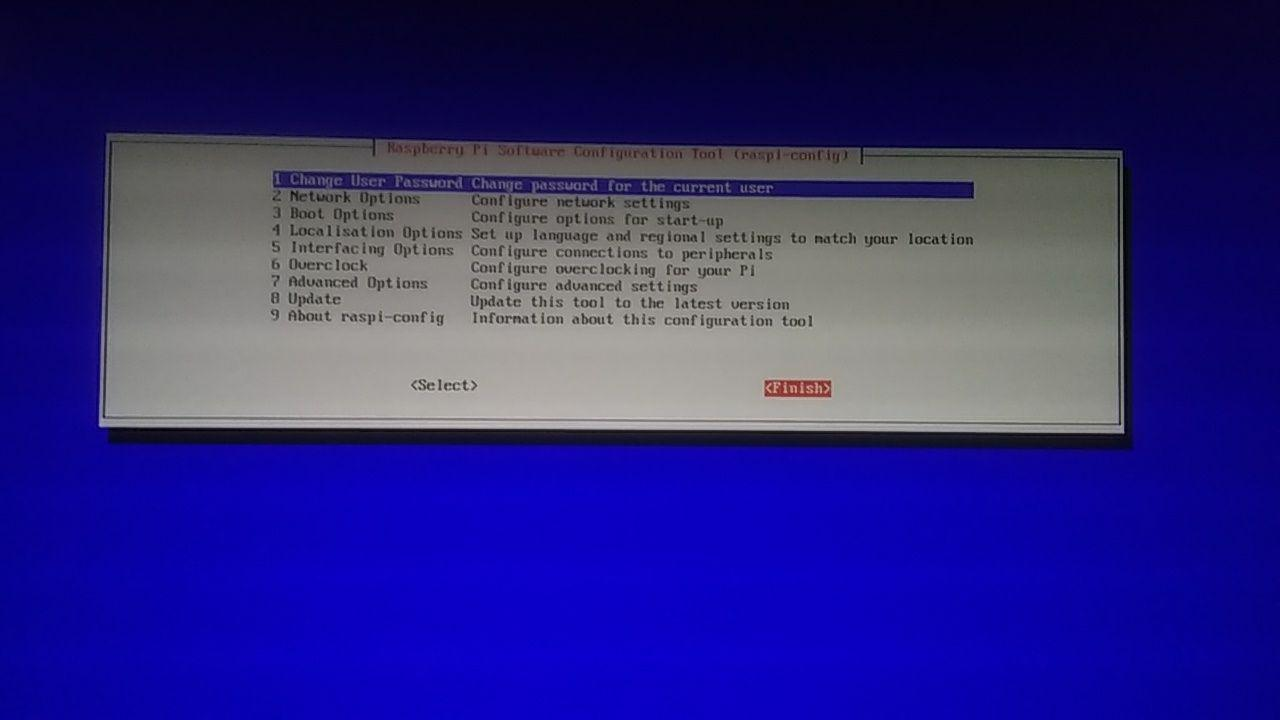
\includegraphics[width=0.75\textwidth]{images/pi/ssh_5.jpg} 
				\caption{The Mikroe Gas Detector}
			\end{figure}
		\subsection{Get the IP address}
			type: \textbf{ip addr} and then enter
			\begin{figure}[ht]
				\centering
				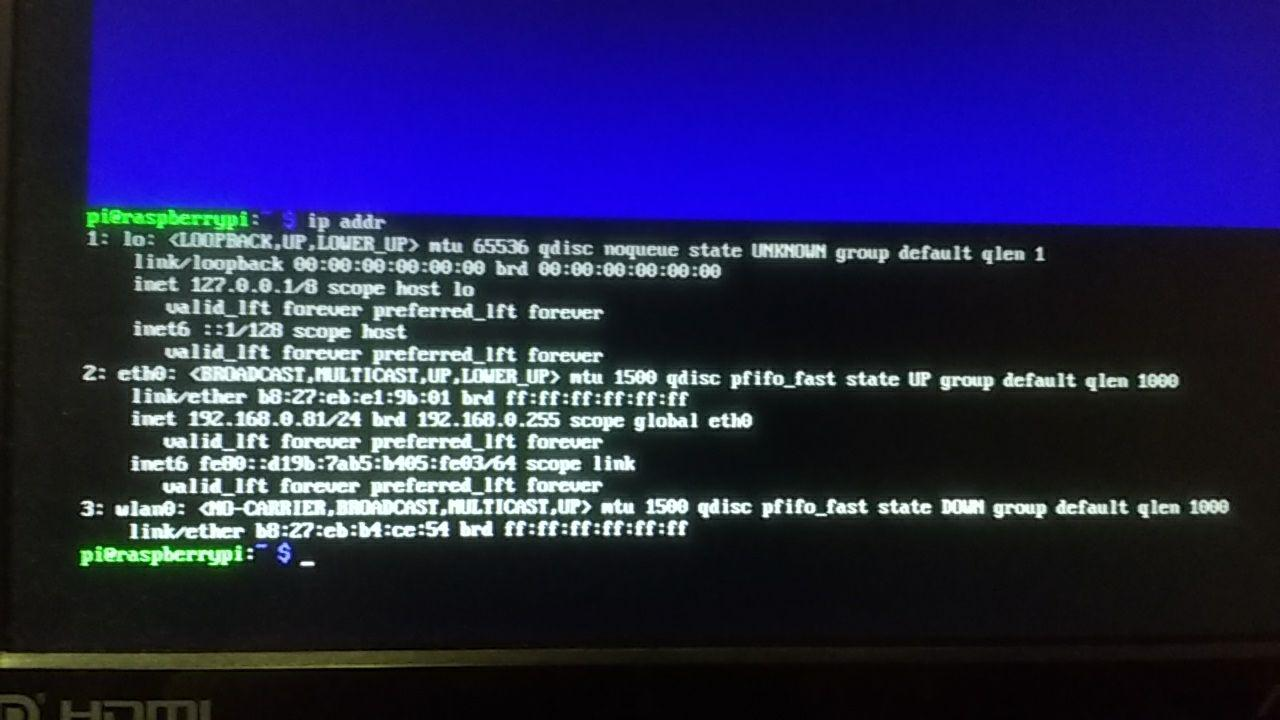
\includegraphics[width=0.75\textwidth]{images/pi/get_ip.jpg} 
				\caption{The Mikroe Gas Detector}
			\end{figure}
			\newpage
		\subsection{Login remotely (Linux or mac)}
			Open your terminal and write 
			\begin{lstlisting}[language=sh]
ssh pi@<<ip-address>>
			\end{lstlisting}
			For example:
			\begin{figure}[ht]
				\centering
				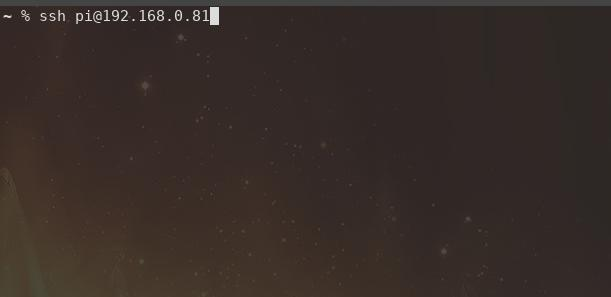
\includegraphics[width=0.75\textwidth]{images/pi/login_ssh_nix.jpg} 
				\caption{The Mikroe Gas Detector}
			\end{figure}\\
			When this is the first connection being made the following question will be asked.
			\begin{figure}[ht]
				\centering
				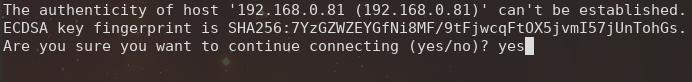
\includegraphics[width=0.75\textwidth]{images/pi/login_ssh_nix_2.jpg} 
				\caption{The Mikroe Gas Detector}
			\end{figure}
			\newpage
			Accept it and, then it will ask for your password (default: raspberry), the typed letters will not show but it will register the characters.
			\begin{figure}[ht]
				\centering
				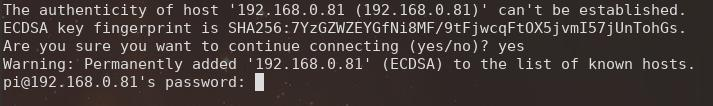
\includegraphics[width=0.75\textwidth]{images/pi/login_ssh_nix_3.jpg} 
				\caption{The Mikroe Gas Detector}
			\end{figure}\\
			When everything went according to the described steps the following screen should be visible:
		\begin{figure}[ht]
			\centering
			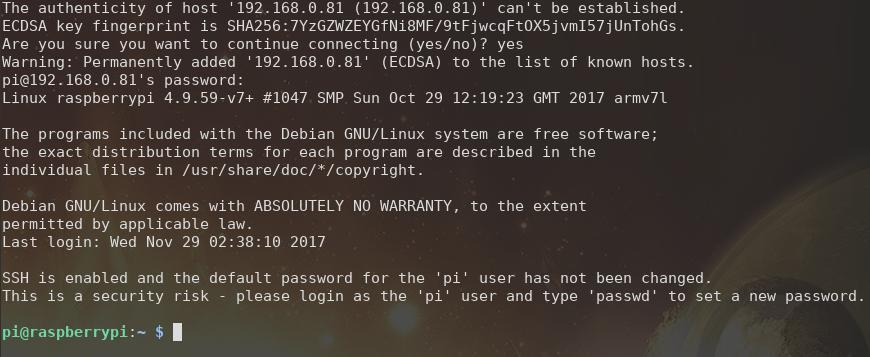
\includegraphics[width=0.75\textwidth]{images/pi/login_ssh_nix_4.jpg} 
			\caption{The Mikroe Gas Detector}
		\end{figure}

		\newpage
	\section{Software}
		After the operating system is installed, the required software must be installed. You do this while being logged in to the Raspberry Pi. Both console or SSH (remote connection) can be used, however the remote connection is advised.
		\subsection{Required packages}
			Install the required base software with the following command (single line).
			\begin{lstlisting}[language=sh]
sudo apt-get -y install network-manager xorg openbox xdm 
	xfce4-terminal xfce4-panel vim dbus-x11 hostapd
	lxappearance numix-gtk-theme git python3-pip feh
	faenza-icon-theme gnome-system-monitor dnsmasq
	python3-pyqt4
			\end{lstlisting}
		\subsection{Install MonitoringBox mangement software}
			\begin{lstlisting}[language=sh]
cd /opt
mkdir MonitoringBox
chmod -c 0777 ./MonitoringBox
git clone git@github.com:pjotrscholtze/MonitoringBox.git ./MonitoringBox
chmod +x /opt/MonitoringBox/Portal/main.py 
pip3 install flask pyserial
mkdir /var/opt/monitoringbox
echo "{}" > /var/opt/monitoringbox/config.json

			\end{lstlisting}

		\subsection{Setup auto login}
			Edit the file
			\begin{lstlisting}[language=sh]
/lib/systemd/system/getty@.service
			\end{lstlisting}
			With for example nano (other editors are also okay):
			\begin{lstlisting}[language=sh]
sudo nano /lib/systemd/system/getty@.service
			\end{lstlisting}
			Change the following line:
			\begin{lstlisting}
ExecStart=-/sbin/agetty --noclear %I $TERM
			\end{lstlisting}
			To the following:
			\begin{lstlisting}
ExecStart=-/sbin/agetty --noclear -a root %I $TERM
			\end{lstlisting}
			(You can save the file with ctrl+o and quite with ctrl+x)\\
			Source: https://superuser.com/questions/969923/automatic-root-login-in-debian-8-0-console-only
		\subsection{Setup better shell (optional)}
			Can be useful when needing to work directly on the device (on the shell if you do not know what that means, than it is most likely not something you are going to use).
			\begin{lstlisting}[language=sh]
apt-get install zsh
chsh -s $(which zsh) pi
sudo chsh -s $(which zsh) root
			\end{lstlisting}
		\subsection{From now on run the commands as root}
		\begin{lstlisting}[language=sh]
sudo -s
cd ~
		\end{lstlisting}
		\subsection{Startup script}
		This isn't used anymore?
			Create the file: 
			\begin{lstlisting}[language=sh]
~/.xinitrc_feh
			\end{lstlisting}
			with for example nano (other text editors are also okay):
			\begin{lstlisting}[language=sh]
sudo nano ~/.xinitrc_feh
			\end{lstlisting}
			And write the following content.
			\begin{lstlisting}[language=sh]
#!/bin/sh
sleep 0.2
feh --bg-fill ~/background.jpg &
			\end{lstlisting}
		/This isn't used anymore?

			Now create the file
			\begin{lstlisting}[language=sh]
~/.xinitrc
			\end{lstlisting}
			with for example nano (other text editors are also okay):
			\begin{lstlisting}[language=sh]
sudo nano ~/.xinitrc
			\end{lstlisting}
			And write the following content in it:
			\begin{lstlisting}[language=sh]
python3 /opt/MonitoringBox/Portal/main.py &
exec openbox-session
\end{lstlisting}
			\paragraph{When \underline{NOT} using ZSH} do the following:
				Append to the
				\begin{lstlisting}[language=sh]
~/.bashrc
				\end{lstlisting}
				file, with for example nano (other text editors are also okay).
				\begin{lstlisting}[language=sh]
sudo nano ~/.bashrc
				\end{lstlisting}
				The following content:
				\begin{lstlisting}[language=sh]
if [ -z "$DISPLAY" ] && [ -n "$XDG_VTNR" ] && 
   [ "$XDG_VTNR" -eq 1 ]; then
  exec startx
fi
				\end{lstlisting}
			\paragraph{When using ZSH} do the following:
				Append to the
				\begin{lstlisting}[language=sh]
~/.zshrc
				\end{lstlisting}
				file, with for example nano (other text editors are also okay).
				\begin{lstlisting}[language=sh]
sudo nano ~/.zshrc
				\end{lstlisting}
				The following content:
				\begin{lstlisting}[language=sh]
if [ -z "$DISPLAY" ] && [ -n "$XDG_VTNR" ] && 
   [ "$XDG_VTNR" -eq 1 ]; then
  exec startx
fi
				\end{lstlisting}
		\subsection{Access point/WiFi setup}
https://frillip.com/using-your-raspberry-pi-3-as-a-wifi-access-point-with-hostapd/
https://superuser.com/questions/985082/is-there-a-way-to-disable-the-dhcp-client-in-raspbian-linux-on-a-rasperry-pi

			\paragraph{Network interface} First setup the network interface (disable DHCP), by editing the following file:
				\begin{lstlisting}[language=sh]
/etc/network/interfaces
				\end{lstlisting}
				With for example nano (other text editors are also okay).
				\begin{lstlisting}[language=sh]
sudo nano /etc/network/interfaces
				\end{lstlisting}
				And make sure the following:
				\begin{lstlisting}
allow-hotplug wlan0  
iface wlan0 inet dhcp @todo
				\end{lstlisting}
				Is changed to the following:
				\begin{lstlisting}
allow-hotplug wlan0  
iface wlan0 inet static  
    address 172.24.1.1
    netmask 255.255.255.0
    network 172.24.1.0
    broadcast 172.24.1.255
				\end{lstlisting}
				And finish with the following commands:
				\begin{lstlisting}
sudo systemctl disable dhcpcd.service
sudo systemctl stop dhcpcd.service
				\end{lstlisting}
				\begin{lstlisting}
---sudo apt-get remove dhcpcd5 @todo check this part
				\end{lstlisting}
				\paragraph{Access point} After the network interface was prepared the access point needs to be setup. First we need to create the following file:
				\begin{lstlisting}
/etc/hostapd/hostapd.conf
				\end{lstlisting}
				Create the directory first:
				\begin{lstlisting}
sudo mkdir /etc/hostapd
				\end{lstlisting}
				Then create the file with for example nano (any other text is also okay).
				\begin{lstlisting}
sudo nano /etc/hostapd/hostapd.conf
				\end{lstlisting}
				And write the following content inside:
				\begin{lstlisting}
# This is the name of the WiFi interface we configured above
interface=wlan0

# Use the nl80211 driver with the brcmfmac driver
driver=nl80211

# This is the name of the network
ssid=Pi3-AP

# Use the 2.4GHz band
hw_mode=g

# Use channel 6
channel=6

# Enable 802.11n
ieee80211n=1

# Enable WMM
wmm_enabled=1

# Enable 40MHz channels with 20ns guard interval
ht_capab=[HT40][SHORT-GI-20][DSSS_CCK-40]

# Accept all MAC addresses
macaddr_acl=0

# Use WPA authentication
auth_algs=1

# Require clients to know the network name
ignore_broadcast_ssid=0

# Use WPA2
wpa=2

# Use a pre-shared key
wpa_key_mgmt=WPA-PSK

# The network passphrase
wpa_passphrase=raspberry

# Use AES, instead of TKIP
rsn_pairwise=CCMP
			\end{lstlisting}
			Now configure the deamon to use the config file. This is done by changing the following file:
			\begin{lstlisting}
/etc/default/hostapd
			\end{lstlisting}
			With for example nano (any other text editor is also okay).
			\begin{lstlisting}
sudo nano /etc/default/hostapd
			\end{lstlisting}
			Change the following line from:			
			\begin{lstlisting}
#DAEMON_CONF=""
			\end{lstlisting}
			\begin{lstlisting}
DAEMON_CONF="/etc/hostapd/hostapd.conf"
			\end{lstlisting}
			Afterwards we need to setup the DNS server so that any address will be forwarded to the PI. This is done by editing the:
			\begin{lstlisting}
/etc/dnsmasq.conf
			\end{lstlisting}
			file with for example nano (any other text editor is also okay).
			\begin{lstlisting}
sudo nano /etc/dnsmasq.conf
			\end{lstlisting}
			And make sure it contains the following content:
			\begin{lstlisting}
interface=wlan0      # Use interface wlan0  
listen-address=172.24.1.1 # Explicitly specify the address to listen on  
bind-interfaces      # Bind to the interface to make sure we aren't sending things elsewhere  
server=8.8.8.8       # Forward DNS requests to Google DNS  
domain-needed        # Don't forward short names  
bogus-priv           # Never forward addresses in the non-routed address spaces.  
dhcp-range=172.24.1.50,172.24.1.150,12h # Assign IP addresses between 172.24.1.50 and 172.24.1.150 with a 12 hour lease time  
address=/#/172.24.1.1
			\end{lstlisting}
			Finally we need to enable the deamons so you can connect to it.
			\begin{lstlisting}
systemctl enable hostapd
systemctl enable dnsmasq
			\end{lstlisting}
		\subsection{Enable remote access (SSH) (optional)}
			The following command will allow you change settings easily on the Pi:
			\begin{lstlisting}
sudo raspi-config
			\end{lstlisting}
			Go to "interfaces" -> SSH and enable the option.
		\subsection{Reduce space consumption (optional)}
			Remove unused packages:
			\begin{lstlisting}[language=sh]
apt-get -y remove bluetooth blackbird-gtk-theme 
	bluebird-gtk-theme scrot samba-common 
	unattended-upgrades xserver-xorg-video-amdgpu 
	xserver-xorg-video-ati xserver-xorg-video-nouveau 
	xserver-xorg-video-radeon xserver-xorg-video-vesa 

apt-get -y purge bluetooth blackbird-gtk-theme 
	bluebird-gtk-theme scrot samba-common 
	unattended-upgrades xserver-xorg-video-amdgpu 
	xserver-xorg-video-ati xserver-xorg-video-nouveau 
	xserver-xorg-video-radeon xserver-xorg-video-vesa 

apt-get -y autoremove
apt-get -y autoclean
			\end{lstlisting}
			\paragraph{Warning} this will remove the unused icons, however this is officially still part of the containing packages so this is not recommended.
			\begin{lstlisting}[language=sh]
rm -rf /usr/share/icons/elementaryXubuntu-dark
rm -rf /usr/share/icons/Faenza-*
			\end{lstlisting}
			\paragraph{Warning} disabling the swap file can lead to unstable performance, however if you use this Raspberry Pi you can safely disable it.
			\begin{lstlisting}[language=sh]
sudo dphys-swapfile swapoff
sudo dphys-swapfile uninstall
sudo update-rc.d dphys-swapfile remove
			\end{lstlisting}

\chapter{Problems and their solutions}
	What to do when you cann't connect to the internet while you've pluggedin the ethernet cable. Run the following command:
	\begin{lstlisting}[language=sh]
sudo service dnsmasq stop
	\end{lstlisting} 
	This will disable DNS and DHCP, thus you cannot connect propperly to the pi via wifi any more but after reboot (or with: sudo service dnsmasq start) you can access it again

\end{document}
